% !TeX spellcheck = en_US

\section{SonarQube}
\subsection{What does SonarQube provide?}
SonarQube offers product metrics for various languages: ABAP, Android, C/C++,
C-Sharp (C\#), COBOL, Flex, Groovy, Java, JavaScript, Objective-C, PHP, PL/I,
PL/SQL, Python, RPG, VB.NET, Visual Basic 6, Web (HTML, JSP/JSF), and XML. In
addition to build-in functionalities, plug-ins allow for multi-language analysis
of code
quality\footnote{\url{http://www.sonarqube.org/at-long-last-sonarqube-is-a-true-polyglot/}}.
It is even possible to compare metrics between different languages and projects,
i.e. side by side comparison between Java and C++.

These are the product metrics currently supported by SonarQube (formerly known
as Sonar)\footnote{\url{http://docs.codehaus.org/display/SONAR/Metric+definitions}}:
\begin{itemize}
	\item \textbf{Cyclomatic Complexity}: overall, and average by class, file and function.
	\item \textbf{Design issues}: 
	\begin{itemize}
		\item cycles, file cycles, file dependencies, and package edge weight, 
		that is, number of dependencies between packages
		\item Depth of inheritance tree (tic)
		\item Number of children (noc) of a class
		\item Response for class (rfc) 
		\item Afferent and efferent couplings (ca, ce): how many classes use 
		this class, or how many classes are used by this class
		\item Lack of cohesion of methods (lcom4), i.e. set of related 
		components of a class. There should be only one, otherwise the class should be divided into smaller classes.
	\end{itemize}
	\item \textbf{Duplications of source code} blocks and lines.
	\begin{figure}[h]
		\centering
		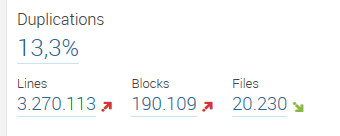
\includegraphics[scale=0.5]{img/code_duplications.jpg}
		\caption{Code duplications per line, block, and file.} 
		\label{fig:code_duplications}
	\end{figure}
	
	\item Metrics about issues: open, confirmed, closed, false positive.
	\item Metrics about defined rule compliance, i.e. violation density. \\
	Violations is the number of rule breaches automatically calculated by
	analyzing the source code of a project. Different projects can be compared to each other. In addition, developers can weight violations to find out where they must start fixing problems first.
	\begin{align}
		\begin{split}
			\label{eq:rules_compliance_index}
			rules\_compliance\_index =&\\
			RCI =& 100 - \frac{weighted\_issues}{LLOC} \cdot 100
		\end{split}
	\end{align}
	\item Technical debt is the effort to fix all issues in minutes.
	\begin{figure}[h]
		\centering
		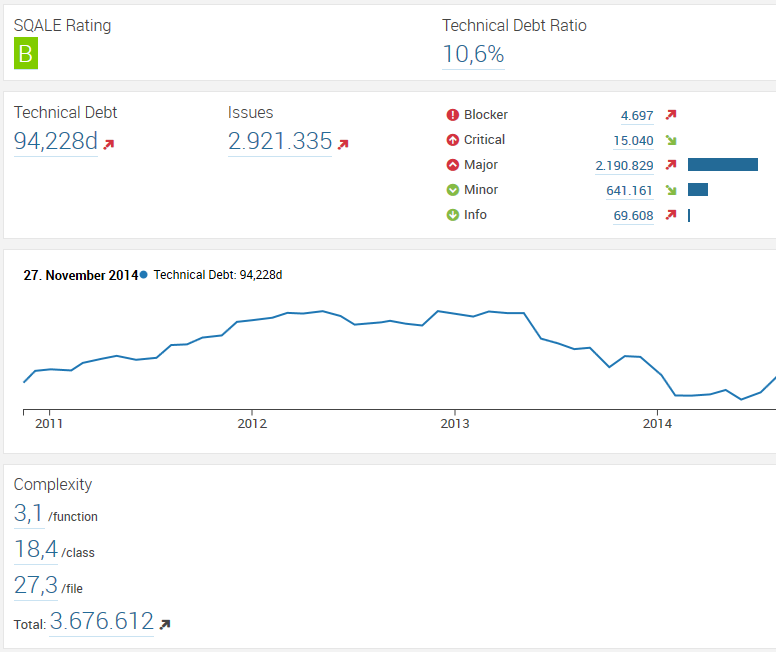
\includegraphics[scale=0.4]{img/technical_debt.jpg}
		\caption{Technical debt and complexity metrics over time} 
		\label{fig:technical_debt}
	\end{figure}
	\item Severity of issues is calculated automatically through defined rules,
	several rule packages already exist for different languages, and are bundled
	together with the default installation.
	\item Size metrics: LLOC, LOC, generated LOC, method counts, class counts, 
	file counts, public API, and statements.
	\item Test metrics: condition coverage for branching code, and separately 
	for new code, and line coverage. Further more it exists a unit test 
	integration with duration, errors, failures, and success density.
	\begin{figure}[h]
		\centering
		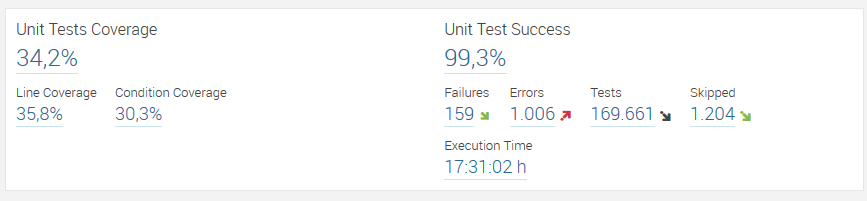
\includegraphics[scale=0.5]{img/unit_test_coverage.jpg}
		\caption{Unit test coverage, success rates and execution time} 
		\label{fig:unit_test_coverage}
	\end{figure}
	\item Documentation metrics: lines of comments, significant lines of comments, commented out production code, and Javadoc support.
	\begin{figure}[h]
		\centering
		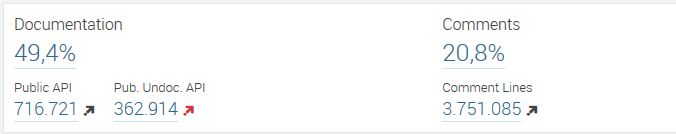
\includegraphics[scale=0.5]{img/documentation.jpg}
		\caption{Metrics about documentation.} 
		\label{fig:documentation}
	\end{figure}
	\item Source code repository metrics about commits, revisions, and authors'
	performance.
\end{itemize}

According to~\cite{Gallaba} the most important metrics are: duplicated blocks, violations,
public undocumented APIs, uncovered complexity by tests, function and class
complexity distribution, and package edge weights.
The overall measures of these metrics are used to calculate the technical debt
in man days:

\begin{align}
	\begin{split}
		\label{eq:technical_debt_in_man_days}
		technical\_debt = & cost\_to\_fix\_duplications + \\
		 	& cost\_to\_fix\_violations + \\
		 	& cost\_to\_comment\_public\_API + \\
		 	& cost\_to\_fix\_uncovered\_complexity + 	\\
		 	& cost\_to\_bring\_complexity\_below\_threshold +\\
		 	& cost\_to\_cut\_cycles\_at\_package\_level
	\end{split}
\end{align}

This technique is known as SQALE Rating\footnote{\url{http://docs.codehaus.org/display/SONAR/Technical+Debt#TechnicalDebt-ComparingprojectswiththeTechnicalDebtRatioandtheSQALERating}}. Technical debt ratio, that is shown in
figure~\ref{fig:technical_debt}, is calculated with the following formula:

\begin{equation}
	\label{eq:technical_debt_ratio}
	technical\_debt\_ratio = technical\_debt / estimated\_development\_cost
\end{equation}

\begin{figure}[h]
	\centering
	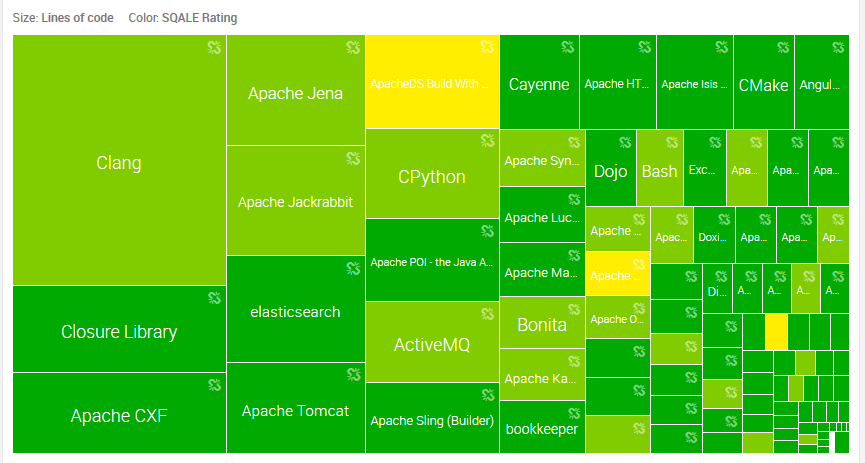
\includegraphics[scale=0.5]{img/sqale_rating.jpg}
	\caption{LOC compared to SQALE Ratings.} 
	\label{fig:sqale_rating}
\end{figure}
	
In addition to these metrics, SonarQube provides Eclipse and IntelliJ plug-ins to
handle issues directly from within the IDEs. It also harvests some state of the
art issue tracker currently available on the market, i.e. JIRA issues, Trac,
Mantis Bug Tracker\footnote{MantisBT is an open source issue tracker:
\url{http://www.mantisbt.org/}}. There exist also plugins to seamlessly include other
test and metric environments, like the Apache JMeter
plugin\footnote{\url{http://docs.codehaus.org/display/SONAR/JMeter+Plugin}} to test
performance of
static and dynamic resources, or Pitest\footnote{PIT is a mutation testing tool for
java: \url{http://pitest.org/}} to handle mutation testing.

\subsection{What can PROM get from SonarQube or add to it?}

\begin{figure}[h]
	\centering
	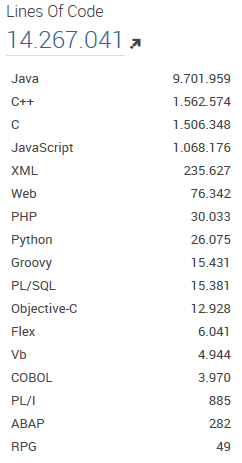
\includegraphics[scale=0.5]{img/lloc.jpg}
	\caption{LOC metric in SonarQube for various languages.} 
	\label{fig:lloc}
\end{figure}

As what I have seen so far, SonarQube is mainly focused on product metrics and
issue tracking environments, i.e. bug reports and task lists. However, I think
it has no effort collection system, since these information is always given
manually by developers. They insert estimates and progressions by hand into
software development management tools, that are harvested later by the SonarQube
analyzing tools, like SonarQube Runner, SonarQube Ant Task, Maven or Gradle
Engines\footnote{How Sonar analyzes source code: \url{http://docs.codehaus.org/display/SONAR/Analyzing+Source+Code}}.

I put the focus to the SonarQube Runner tool for the moment, since it is the
recommended analyzer.  This tool analyzes a project and puts all calculated
metrics into a specified database. 

First, we could use this data to enhance PROM's feature list, with the metrics
mentioned earlier in this document.
Second, PROM could add real-time effort data to imported task structures and
issues. That is, combine effort accumulated by a developer per task. These tasks
could then, also with PROM, be combined with source code fragments, i.e.
classes, methods, name spaces, and projects. The capability of SonarQube to
provide a list with the most critical project components, that is components
that have a high probability to fail, combined with real effort data connected
to them, could provide powerful statistics. For example, if a developer
estimated a task with X man days and worked on it for a certain time Y, an
effort analysis plug-in that accesses PROM data, could provide real-time
''technical debt'' or ''print completion'' (i.e., for SCRUM methodology)
statistics. On one hand, we could provide such statistics for tasks and issues.
On the other hand, we could provide them for source code fragments.

Another feature, that we could use to extend PROM, are source code complexity
metrics. The PROM team implemented some metrics for source code analysis. These
are, CBO (coupling between objects),  CC (cyclomatic complexity), DIT (Depth of
Inheritance Tree), LCOM (lack of cohesion of methods), NOC (number of children),
RFC (response set of a class), and WMC (weighted methods for class), and more
direct metrics like LOC, and LLOC. However, these metrics work only (as I know)
for Java and C++. SonarQube provides most of these metrics for a broad variety
of languages, as you can see in figure~\ref{fig:lloc}.

\subsection{Suggestions for plug-ins}

\subsubsection{First plug-in: Combine effort data with source code}

First, I would suggest to integrate non-invasive effort metrics to projects that
SonarQube manages. That is, map effort to source code fragments. 

A possible outcome could be a table that shows the overall effort of a project,
and on higher granularity it provides effort subdivided into name spaces,
classes, and methods. Since SonarQube allows to import source code from revision
control systems, like GIT or SVN, it would be important to add revisions to such
metrics as well. This is, as I know, not implemented yet for PROM.

\subsubsection{Second plug-in: Combine effort data with tasks and issues}

Second, I would suggest to create a visualization plug-in that shows non-invasive
effort metrics per task and issue. We could also add PERT or GANTT to gain
additional value. To provide a professional state-of-the-art tool, that supports
third-party products we could also create an export function, i.e. for Microsoft
Project. However, SonarQube is an open-source tool, I think it would be better
to export data to other open-source management tools, like GanttProject. I have
done such a project for my Bachelor thesis. It is possible to reuse this as a
SonarQube plugin.

\subsubsection{Third plug-in: Integrate PROM's GQ(I)M dashboard}

Third, SonarQube has no support for a GQM dashboard. I think, developers will
appreciate if we create a SonarQube GQ(I)M dashboard to visualize their
statistics enriched with our effort metrics. 

All three plugins could be combined to a PROM suite for SonarQube. In general,
we should provide some REST interface, to simply query PROM's effort collections
according to certain filters and constraints. However, this would involve some
major project changes and improvements.
